\section{DNA Thermodynamics}

\begin{figure}[ht]
  \begin{centering}
  \adjustbox{minipage=1.3em,valign=t}{\subcaption{}\label{sfig:testa}}%
  \hspace{-0.3cm}
  \begin{subfigure}[t]{\dimexpr.2\linewidth-1.3em\relax}
  \centering
  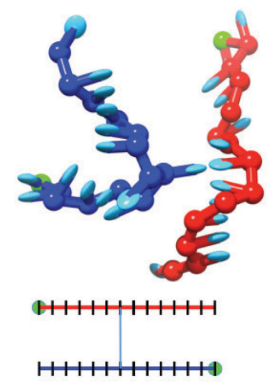
\includegraphics[width=1.06\linewidth,valign=t]{Figures/hybridDiag1.png}
  \end{subfigure}%
  \adjustbox{minipage=1.3em,valign=t}{\subcaption{}\label{sfig:testa}}%
  \hspace{-0.35cm}
  \begin{subfigure}[t]{\dimexpr.2\linewidth-1.3em\relax}
  \centering
  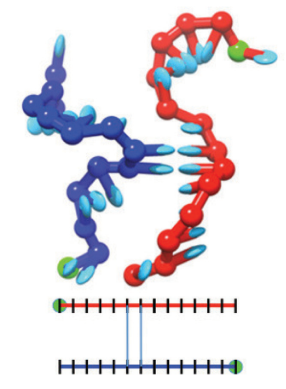
\includegraphics[width=1.09\linewidth,valign=t]{Figures/hybridDiag2.png}
  \end{subfigure}%
  \adjustbox{minipage=1.3em,valign=t}{\subcaption{}\label{sfig:testb}}%
  \hspace{-0.28cm}
  \begin{subfigure}[t]{\dimexpr.2\linewidth-1.3em\relax}
  \centering
  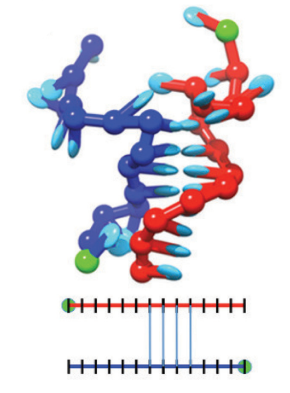
\includegraphics[width=1.1\linewidth,valign=t]{Figures/hybridDiag3.png}
  \end{subfigure}
  \adjustbox{minipage=1.3em,valign=t}{\subcaption{}\label{sfig:testa}}%
  \hspace{-0.21cm}
  \begin{subfigure}[t]{\dimexpr.2\linewidth-1.3em\relax}
  \centering
  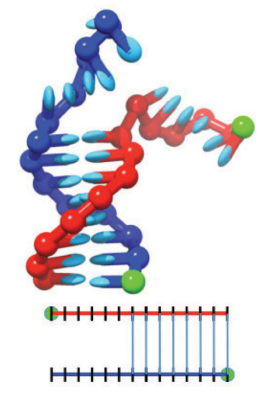
\includegraphics[width=.98\linewidth,valign=t]{Figures/hybridDiag4.png}
  \end{subfigure}%
  \adjustbox{minipage=1.3em,valign=t}{\subcaption{}\label{sfig:testa}}%
  \hspace{-0.38cm}
  \begin{subfigure}[t]{\dimexpr.2\linewidth-1.3em\relax}
  \centering
  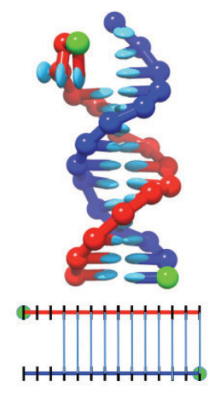
\includegraphics[width=.8\linewidth,valign=t]{Figures/hybridDiag5.png}
  \end{subfigure}
  % \adjustbox{minipage=1.3em,valign=t}{\subcaption{}\label{sfig:testb}}%
  % \hspace{-0.5cm}
  % \begin{subfigure}[t]{\dimexpr.2\linewidth-1.3em\relax}
  % \centering
  % 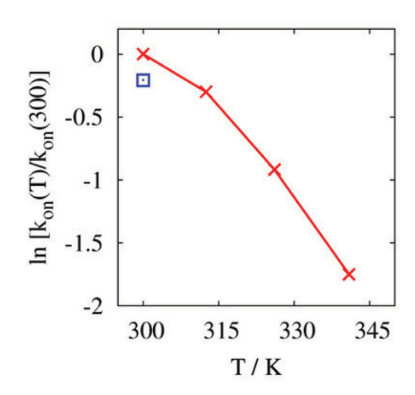
\includegraphics[width=1.5\linewidth,valign=t]{Figures/hybridDiag6.png}
  % \end{subfigure}
  \caption{This is a figure [.]}
  \label{fig:test}
  \end{centering}

\end{figure}


\newpage



 The field of DNA thermodynamics focuses on understand how the structure of DNA varies
 with temperature. Due to nature of the hydrogen bond interactions that give rise to the
structure of dsDNA, the association and dissociation of the DNA duplex is possible. The
former is called DNA hybridisation, which is driven by a reduction in free energy due to
the bonding of complementary base-pairs. While the latter is called DNA melting, a
process seen at high temperatures, where the trade-off in configurational entropy during
duplex formation is no longer favourable compared to the reduction in free energy.

During the discussion of the DNA nanopiston, we stated that thermodynamic transitions are
the driving force behind its operating cycle. The power stroke in the cycle is induced by
a toehold mediated strand displacement reaction, while a hybridisation reaction
facilitates the recovery stroke.


Initiating strand hybridisation reaction incurs a thermodynamic penalty, this penalty
originates in the decrease of configurational entropy when the strand start to form a
duplex. This has a consequence that initial contacts in these reactions often dissociate.
Even when an initial contact results in the stabilisation of the duplex for select
base-pairs, the configuration often times is not conducive to full duplex formation.

The main reasons is that these transitions are not characterised by a single state but
rather by a ensemble of possible transition pathways. The number of pathways increase
dramatically when the strand sequences are repetitive, giving rise to hybridisation
pathways called the Inchworm and the pseudo knot.

The combination of  unstable initialisation of the hybridisation reaction together with
the many transition pathways complicates the study of hybridisation with MD simulations

Deze nog ergens gebruiken:

‘fraying’ to describe the disruption of base pairs at the end of a duplex; if all base
pairs fray, the duplex melts or dissociates.

‘zippering’ refers to when a new base pair forms at the end of an existing duplex, shown
in figure 3.2

-----------------------------------------------------------------------------------------

The other important thermodynamic transition is the Toehold mediated strand displacement.
This reaction involved three DNA strand, of which two partially complementary strands
from an imperfect duplex structure. The two strands can be partially complementary by
having either a mismatch in basepair or a number of basepairs. The non hybridised part of
the strand constitutes a flexible ssDNA strand that is refered to as the toehold.

The third strand in this reaction is fully complementary with one of the strands in the
duplex, making it energetically favourable for the .

strand displacement increases number of hybridised base pairs, fully Watson–Crick
complementary -> descreasing the overall free energy of the system. Overall, displacement
is thermodynamically driven forward by the net gain in base pairs due to the toehold


Once the toehold has bound, there are two possibilities: (i) the toehold base pair could
dissociate, leading to the dissoci- ation of the invader or (ii) the nearest base pair of
the substrate-incumbent complex could fray, allowing the invader to compete to replace
that base pair and complete the first step of branch migration.

as may seem reasonable, that the rate at which either base pair frays is similar, process
(ii) should be approximately half as fast as process (i).  strand displacement kinetics
depends on toehold length.  Intiating strand displacement incurs a thermodynamic penalthy
(making is difficult to simulate).

This is because, once the substrate- incumbent base pair frays, there is a 50% chance of
the invader replacing the frayed base pair, and a 50% chance of returning to the initial
step.

Therefore, the probability of successfully completing the remaining steps ofbranch
migration before going back to the toehold-only- bound state is 1/20, from the gambler’s
ruin analysis

model branch migration at a more detailed level. we analyze a 1D (single-pathway) model
of toehold-mediated strand displacement called the intuitive energy landscape (IEL) model
-> refer to graph on image.

-----------------------------------------------------------------------------------------

Conclusion: Reactions do not happen that easy, difficult to simulate, especially the
toehold displacement reaction. An advanced sampling technique is needed to sample these
rare events.

\begin{figure}[ht]
\begin{center}
  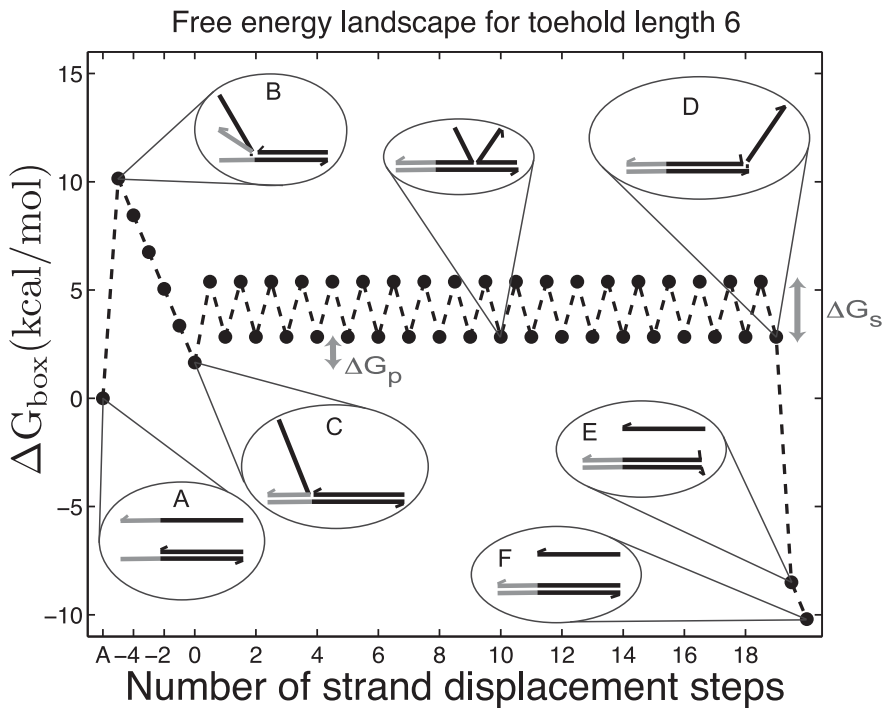
\includegraphics[width=0.5\textwidth]{Figures/ToeholdDiagram.png}
  \caption{write caption[.]}
\end{center}
\end{figure}


